\documentclass{diploma}

\student{Ядров Артем Леонидович}
\group{М8О-408Б-20}
\theme{Создание системы преобразования рукописного математического текста в LaTeX}

\supervisor{Миронов Евгений Сергеевич}
\firstConsultant{Кондаратцев Вадим Леонидович}
\secondConsultant{---}
\reviewer{---}

\faculty{№ 8 <<Компьютерные науки и прикладная математика>>}
\department{806}
\speciality{01.03.02 <<Прикладная математика и информатика>>}
\profile{Информатика}

% Здесь необходим разрыв строки из-за особенностей титульной страницы
\departmentFullName{№ 806}
\headOfDepartment{Крылов Сергей Сергеевич}

% Дата. Оставляем пустое место для дня
\date{\uline{\hspace{24pt}} мая \the\year\ года}

% \newglossaryentry{latex}{
    name={\LaTeX},
    description={система компьютерной вёрстки, широко используемая для создания научных и технических документов. Она основана на языке разметки TeX, созданном Дональдом Кнутом, и включает в себя множество макросов и стилей, которые облегчают работу с текстом и форматирование документов}
}

\newglossaryentry{true_positives}{
    name={True Positives (TP)},
    description={количество правильных предсказаний положительного класса}
}

\newglossaryentry{false_positives}{
    name={False Positives (FP)},
    description={количество неправильных предсказаний положительного класса (когда модель предсказывает положительный класс, а на самом деле объект принадлежит к отрицательному классу)}
}

\newglossaryentry{precision}{
    name={Precision},
    description={одна из метрик машинного обучения, используется для оценки точности модели в отношении положительных предсказаний. 
    Вычисляется по формуле как отношение количества правильных предсказаний положительного класса к общему количеству предсказаний положительного класса}
}
% \newacronym{map}{mAP}{Mean Average Precision}

\newacronym{iou}{IoU}{Intersection over Union}

\newacronym{pdf}{PDF}{Portable Document Format}

\newacronym{dvi}{DVI}{Device Independent file format}

\newacronym{grpc}{GRPC}{Google Remote Procedure Call}

\newacronym{api}{API}{Application Programming Interface}

\addbibresource{main.bib}

% Иллюстрации всегда по центру
\makeatletter
\g@addto@macro\@floatboxreset\centering
\makeatother
    
\begin{document}
\maketitle

% \includepdf[pages=-]{extra/task} % Задание
\setcounter{page}{2} % Устанавливает счётчик страниц

% \abstract

\keywords{ОБРАБОТКА ИЗОБРАЖЕНИЙ, РАСПОЗНАВАНИЕ ТЕКСТА, МАШИННОЕ ОБУЧЕНИЕ, НЕЙРОННЫЕ СЕТИ}

Объектом исследования в данной работе является научный текст и способы его обработки.

Цель работы –-- разработка платформы, выполняющей распознавание научного текста и  генерацию готового \LaTeX--кода.

Основное содержание работы состояло в разработке алгоритма распознования формул на изображении научного текста и последующей генерации \LaTeX--кода данного текста.

Основными результатами работы, полученными в процессе разработки, является обученная для поиска формул на изображении нейросетевая модель, модуль для генерации \LaTeX--кода.

Результаты разработки предназначены для автоматического преобразования научного текста в \LaTeX--код.

Использование результатов данной работы позволяет сократить время верстки научного документа, а также оцифровывать отсканированные источники. % Реферат

\tableofcontents % Содержание 
\termsanddefenitions % Термины и определения
\listofabbreviations % Перечень сокращений и обозначений

\introduction % Структурный элемент: ВВЕДЕНИЕ

В России на постоянной основе проводятся научные исследования во многих областях. Результаты этих исследований публикуются в виде научных статей, которые являются важным инструментом для распространения новых знаний и научных открытий.
Например, по данным "Научной электронной библиотеки"\;опубликовано 52573694 \cite{eLib} статей, и большинство из них написано с помощью \LaTeX ~--- мощного инструмента для верстки и оформления математических формул и научных текстов, который позволяет создавать качественные и профессионально оформленные статьи. 
Также с помощью \LaTeX\; можно готовить конспекты к предметам, причем это может делать как преподаватель, так и студент.

Так как \LaTeX ~--- система верстки со своим особенным синтаксисом, то набор даже простых формул в нем может оказаться сложным процессом. Покажем весь процесс написания \LaTeX--кода на следующем простом примере
\begin{equation}
    \label{formula_example}
        f(x,y,\alpha, \beta) = \frac{\sum \limits_{n=1}^{\infty} 
        A_n \cos \left( \frac{2 n \pi x}{\nu} \right)} {\prod \mathcal{F} {g(x,y)} } 
\end{equation}

На рисунке ~\ref{formula_listing} показан листинг \LaTeX--кода формулы \ref{formula_example}:

\begin{figure}
    \begin{lstlisting}[language={[LaTeX]Tex}]
        f(x,y,\alpha, \beta) = \frac{
            \sum \limits_{n=1}^{\infty} A_n \cos 
            \left( \frac{2 n \pi x}{\nu} \right)
            } {
                \prod \mathcal{F} {g(x,y)} 
            } 
    \end{lstlisting}
    \caption{Листинг формулы ~\ref{formula_example}}
    \label{formula_listing}
\end{figure}

На данном листинге мы наблюдаем большое разнообразие команд \LaTeX. 
Все команды в \LaTeX\; начинаются со знака '\textbackslash', аргументы команд должны заключаться в фигурные скобки '\{\}',
а опции команды --- в квадратные '[]'. Также на листинге приведен пример вложенности команд друг в друга. 
Данные особенности усложняют не только чтение, но и в первую очередь написание кода документа.

После написания исходного кода документа, необходимо произвести компиляцию в один из поддерживаемых форматов: $\textit{.pdf}$ и $\textit{.dvi}$. 
На данном этапе отсеиваются все синтаксические ошибки, компилятор укажет (не всегда однозначно и понятно) на них в логе. 
Однако, такие ошибки как пропущенный или неправильно написанный символ, выравнивание и пр. не являются синтаксическими, и обнаружить их можно лишь при просмотре готового документа. 
После исправления ошибки необходимо заново компилировать документ, что увеличивает время написания документа.

Автоматическая генерация \LaTeX\--кода позволит сократить количество компиляций и уменьшить допускаемые человеком ошибки в написании формул, что ускорит процесс верстки документов.

Также существует множество источников, оцифрованных в форматы $pdf$, $djvu$ и др. 
Хранение в отсканированном виде источников обладает недостатками, такими как невозможность поиска по тексту и быстрого перемещения по нему.
Возможность преобразовывать данные файлы в \LaTeX--код позволит получить данные источники в оцифрованном, а не отсканированном виде, что устранит приведенные недостатки.

Стоит отметить, что уже существуют решения, позволяющие выполнять генерацию \LaTeX--кода по изображению, например, $Mathpix$ \cite{mathpix}. Однако, данное решение обладает рядом недостатков:
\begin{itemize}
    \item распространение по платной подписке;
    \item отсутствие открытого исходного кода;
    \item ограниченная поддержка языков: основным поддерживаемым языком является английский.
\end{itemize}

В настоящее время появляется все больше различных нейросетей (например, Гигачат \cite{gigachat}, ChatGPT \cite{chat_gpt}, Midjourney \cite{midjourney} и тд). Некоторые из них обучены под задачи распознавания текста, в том числе математического. 
Также существуют модели, способные генерировать готовый код. 

На основании вышенаписанного возникает идея автоматизации процесса преобразования научного текста на изображении в готовый \LaTeX--код.


Целью работы является разработка платформы, выполняющей распознавание научного текста и  генерацию готового \LaTeX--кода.

Для достижения поставленной цели в работе были решены следующие задачи:
\begin{itemize}
    \item определение пользовательских сценариев;
    \item определение требований к платформе;
    \item проектирование архитектуры платформы;
    \item разработка сервиса для распознавания научного текста;
    \item разработка сервиса для синхронизации локальных и облачных пользовательских данных;
    \item разработка настольного приложения для взаимодействия пользователя с сервером;
    \item тестирование и анализ прототипа платформы.
\end{itemize}

Для разработки программного обеспечения необходимо изучить технологии и методы, решающие поставленные задачи. Работа основывается на следующих библиотеках, технологиях, алгоритмах:
\begin{itemize}
    \item $Python$ является основным языком программирования, который использовался для решения задач;
    \item $Tensorflow$ --- библиотека для запуска и обучения моделей;
    \item $YOLO$ --- модель, созданная для классификации объектов на изображении;
    \item $OpenCV$ --- библиотека для обработки изображения;
    \item $tkinter$ --- $Python$ библиотека для работы с $GUI$;
    \item $grpc$ --- фреймворк для удаленного вызова процедур;
    \item $\textit{Weights \& Biases}$ --- сервис для отслеживания метрик обучения.
\end{itemize}

Результатом работы является:
\begin{itemize}
    \item сервис для коррекции перспективы изображения;
    \item сервис для нахождения формул на изображении;
    \item дообученная модель $YOLO$, позволяющая находить формулы на изображении;
    \item сервис для преобразования найденных формул в \LaTeX-код;
    \item настольное приложение с авторизацией в $Google\; Drive$ и взаимодействием с удаленным сервером с помощью $grpc$.
\end{itemize} % Введение

% \section{ПОСТАНОВКА ЗАДАЧИ И ТЕОРЕТИЧЕСКИЕ ПРЕДПОСЫЛКИ}

Итак, перед нами стоит задача разработки прототипа платформы, позволяющей преобразовывать изображение с математическим текстом в \LaTeX-код.

\subsection{Пользовательские сценарии}
Для того, чтобы определить требования к нашей платформе, были проработаны пользовательские сценарии.

Для начала определим основные роли целевых пользователей:
\begin{enumerate}
    \item Пользователь мобильного приложения
    \item Пользователь $desktop$ приложения
    \item Пользователь $web$ приложения
    \item Программист
\end{enumerate} % Глава 1
\section{РАЗРАБОТКА ПРОГРАММНОГО ПРОДУКТА}

Конечный продукт является целостной системой, и необходимо рассказать про каждую ее часть. Пожалуй, стоит начать с самой главной ее части - нейросетевой.
\subsection{Высокоуровневая архитектура нейронной сети}

Поскольку преобразование изображения в текст нетривиальная задача, было решено разбить её на несколько модулей. Каждый из модулей можно охарактеризовать входными данными и результатом работы модуля (выходными данными).
Такой подход обладает рядом преимуществ:
\begin{enumerate}
    \item Гибкость и масштабируемость: Модульная структура позволяет легко добавлять новые компоненты или модифицировать существующие без необходимости переписывать всю модель.
    \item Ускорение процесса обучения: Благодаря возможности параллельной обработки данных, модульные нейронные сети обучаются быстрее, чем монолитные модели.
    \item Улучшение качества модели: Разделение модели на модули позволяет специалистам сосредоточиться на оптимизации каждого компонента, что в итоге приводит к улучшению общей производительности модели.
    \item Простота внедрения новых технологий: Модульная архитектура облегчает внедрение новых технологий и подходов, таких как трансфертное обучение или диффузионные модели.
    \item Улучшение производительности: некоторые модули могут исполняться в препроцессинге на клиентской машине, что ослабляет нагрузку на сервер.
\end{enumerate}
Однако, имеются и недостатки:
\begin{enumerate}
    \item Проблемы с совместимостью: Разные модули могут использовать различные архитектуры, форматы данных и методы обучения, что может привести к проблемам совместимости.
    \item Риск ухудшения производительности: Неправильно спроектированные или плохо интегрированные модули могут снизить общую производительность модели.
    \item Необходимость в дополнительных ресурсах: Для обучения и развертывания модульных моделей часто требуются дополнительные ресурсы, такие как GPU или TPU.
\end{enumerate}

Несмотря на недостатки, в современных реалиях важно уметь быстро и без проблем масштабироваться и заменять при необходимости один компонент другим, поэтому было принятно решение использовать модульную архитектуру.
Такая представлена на рисунке ~\ref{neuro_model}

\begin{figure}
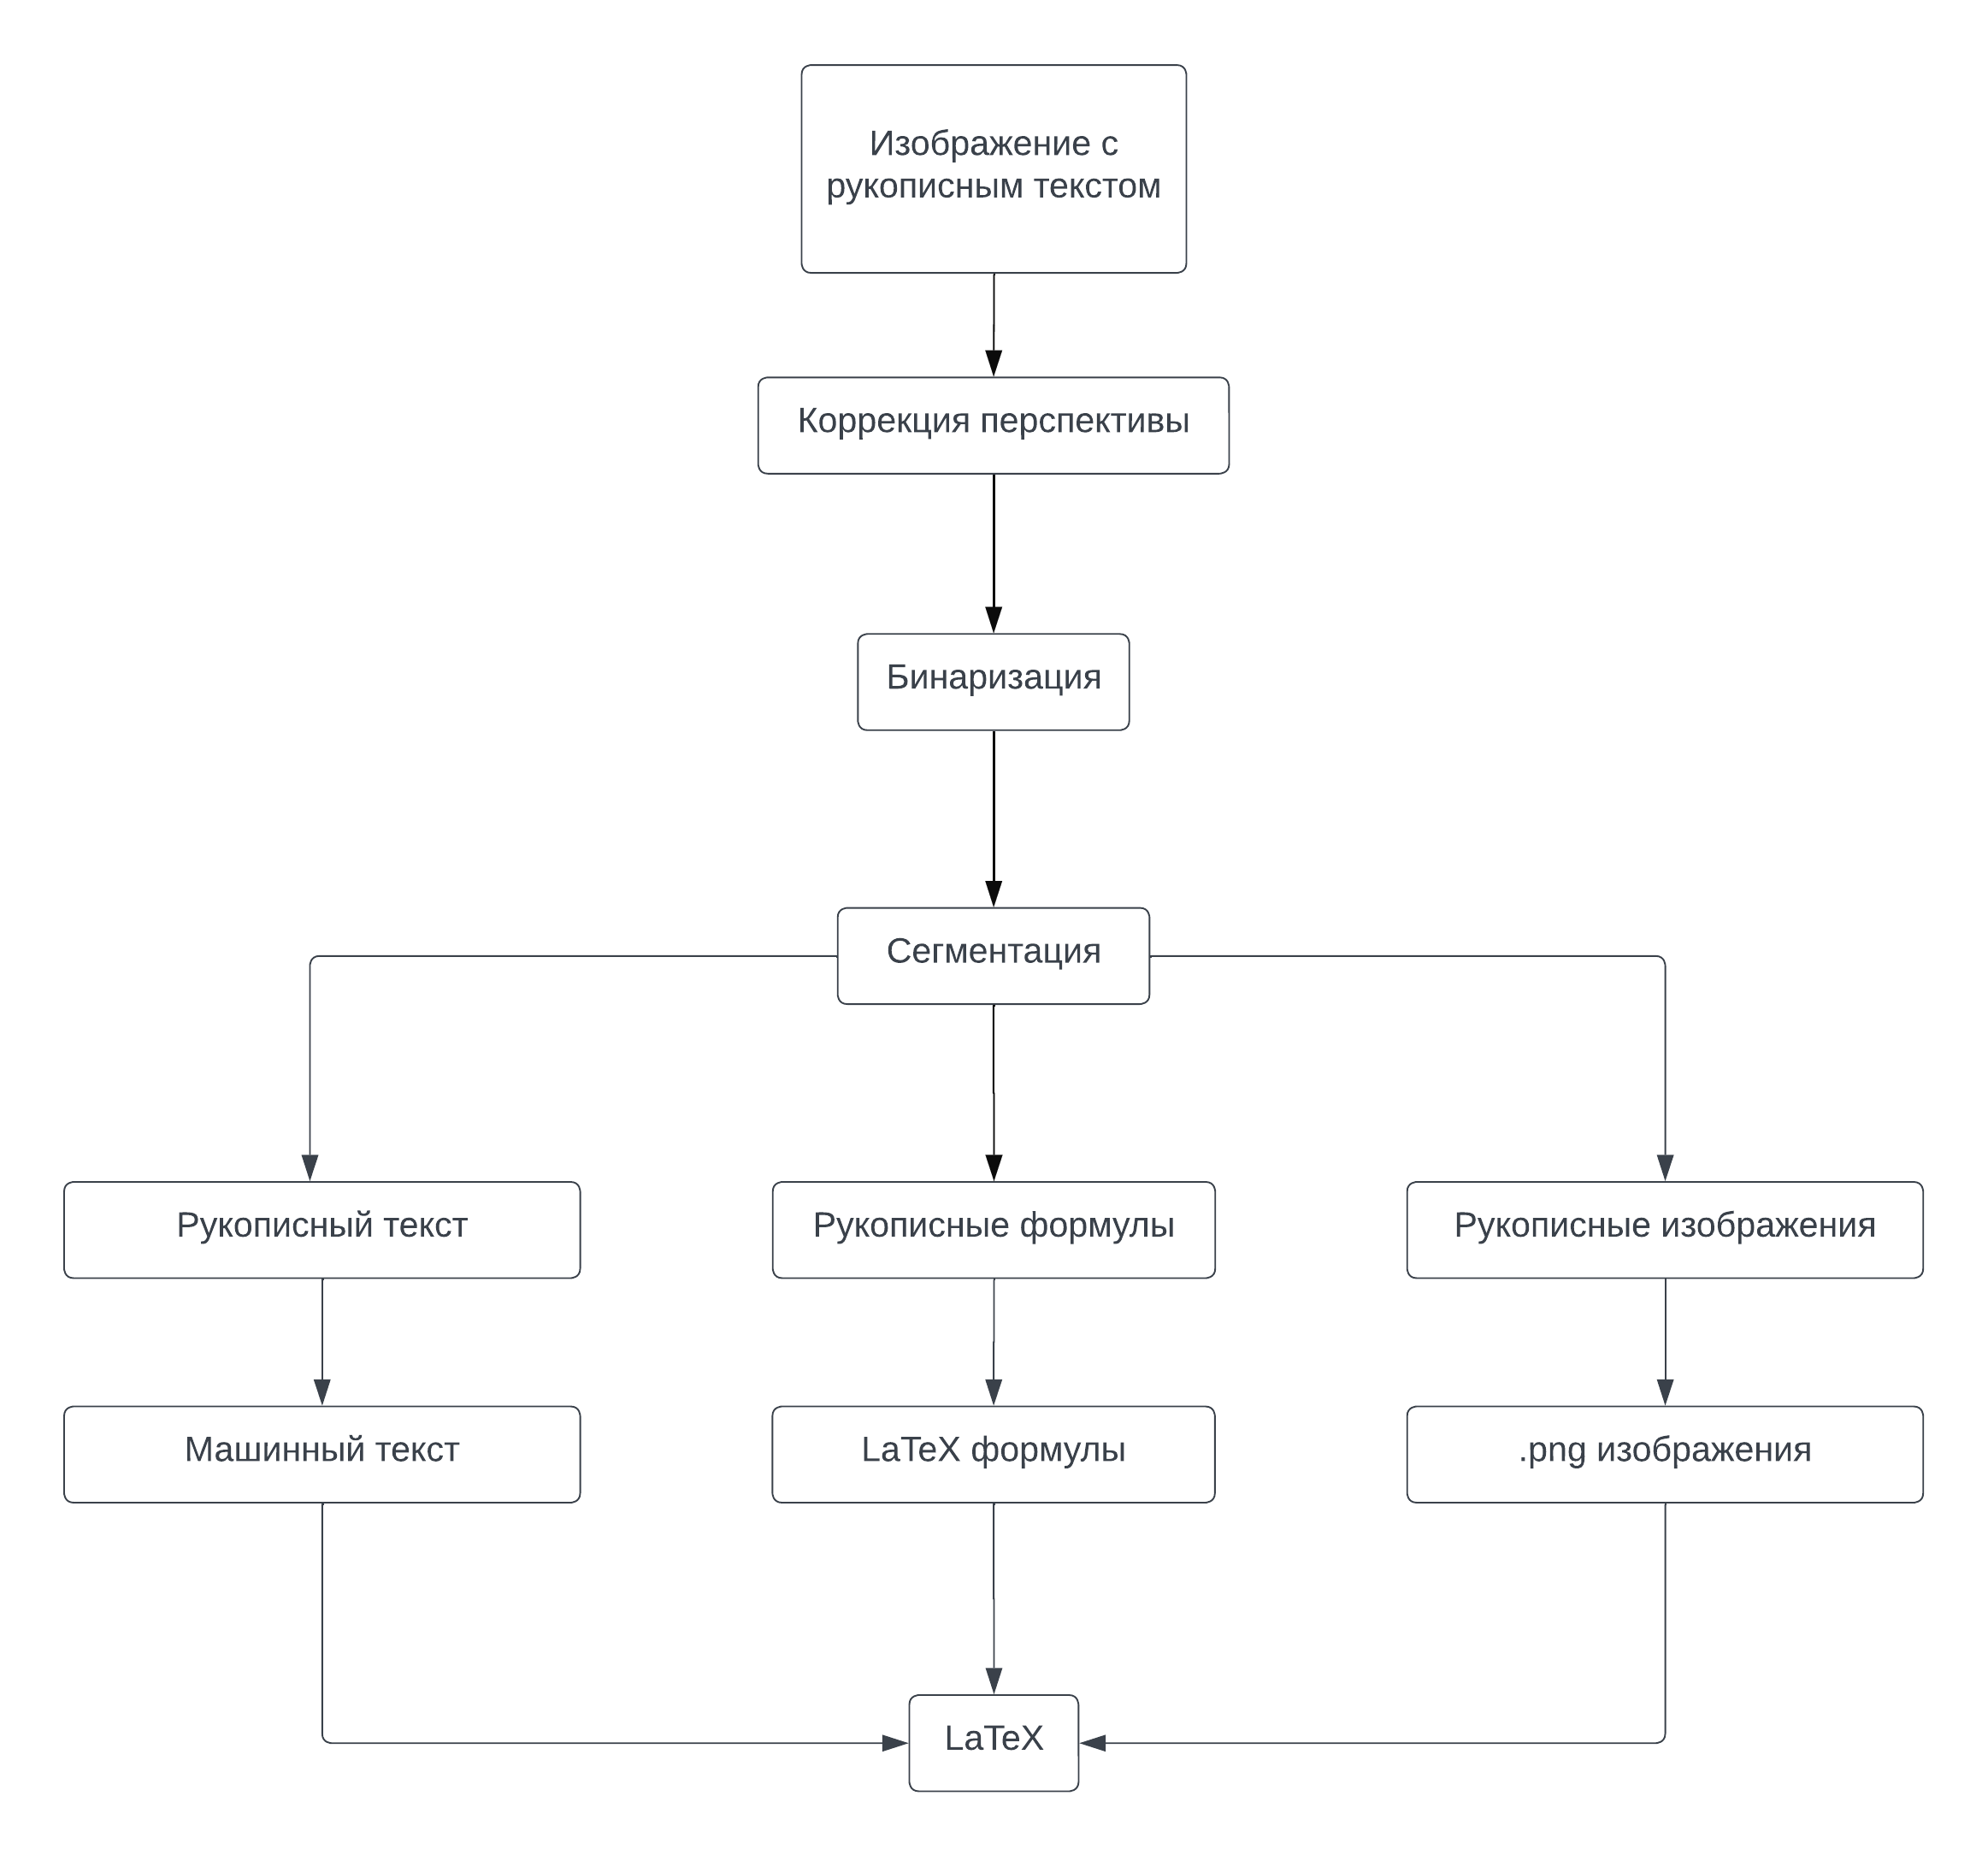
\includegraphics[scale=0.75]{img/Blank_diagram.png}
\caption{Общая архитектура модели}
\label{neuro_model}
\end{figure}

Подробнее разберем каждый этап данной схемы.
\subsection{Коррекция перспективы}

Коррекция перспективы необходима для устранения шума на изображении и получения лучшего результата. Она состоит из нескольких этапов, представленных на рисунке ~\ref{perspective_correction_algo}. 
Также на рисунке представлены результаты, получаемые на каждом из этапов обработки.

Стоит отметить, что коррекция перспективы осуществляется с использованием только алгоритмов обработки изображения без использования каких-либо нейросетей. 
Поэтому в целях экономии ресурсов сервера, а в следствии улучшения производительности было принято решение выполнять данный этап на машине клиента.
Схема данного алгоритма представлена на рисунке ~\ref{perspective_correction_algo}.
\begin{figure}
    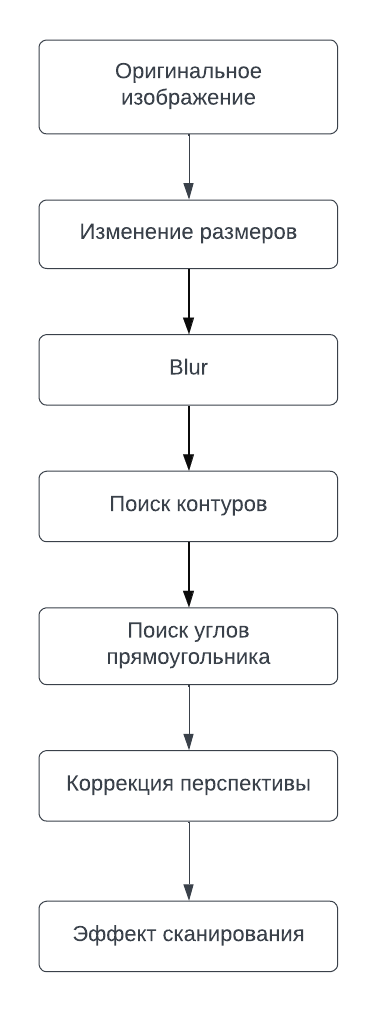
\includegraphics[scale=0.75]{img/perspective_correction}
    \caption{Этапы коррекции перспективы изображения}
    \label{perspective_correction_algo}
\end{figure}

На начальном этапе мы имеем изображение, показанное на рисунке ~\ref{input}

\begin{figure}
    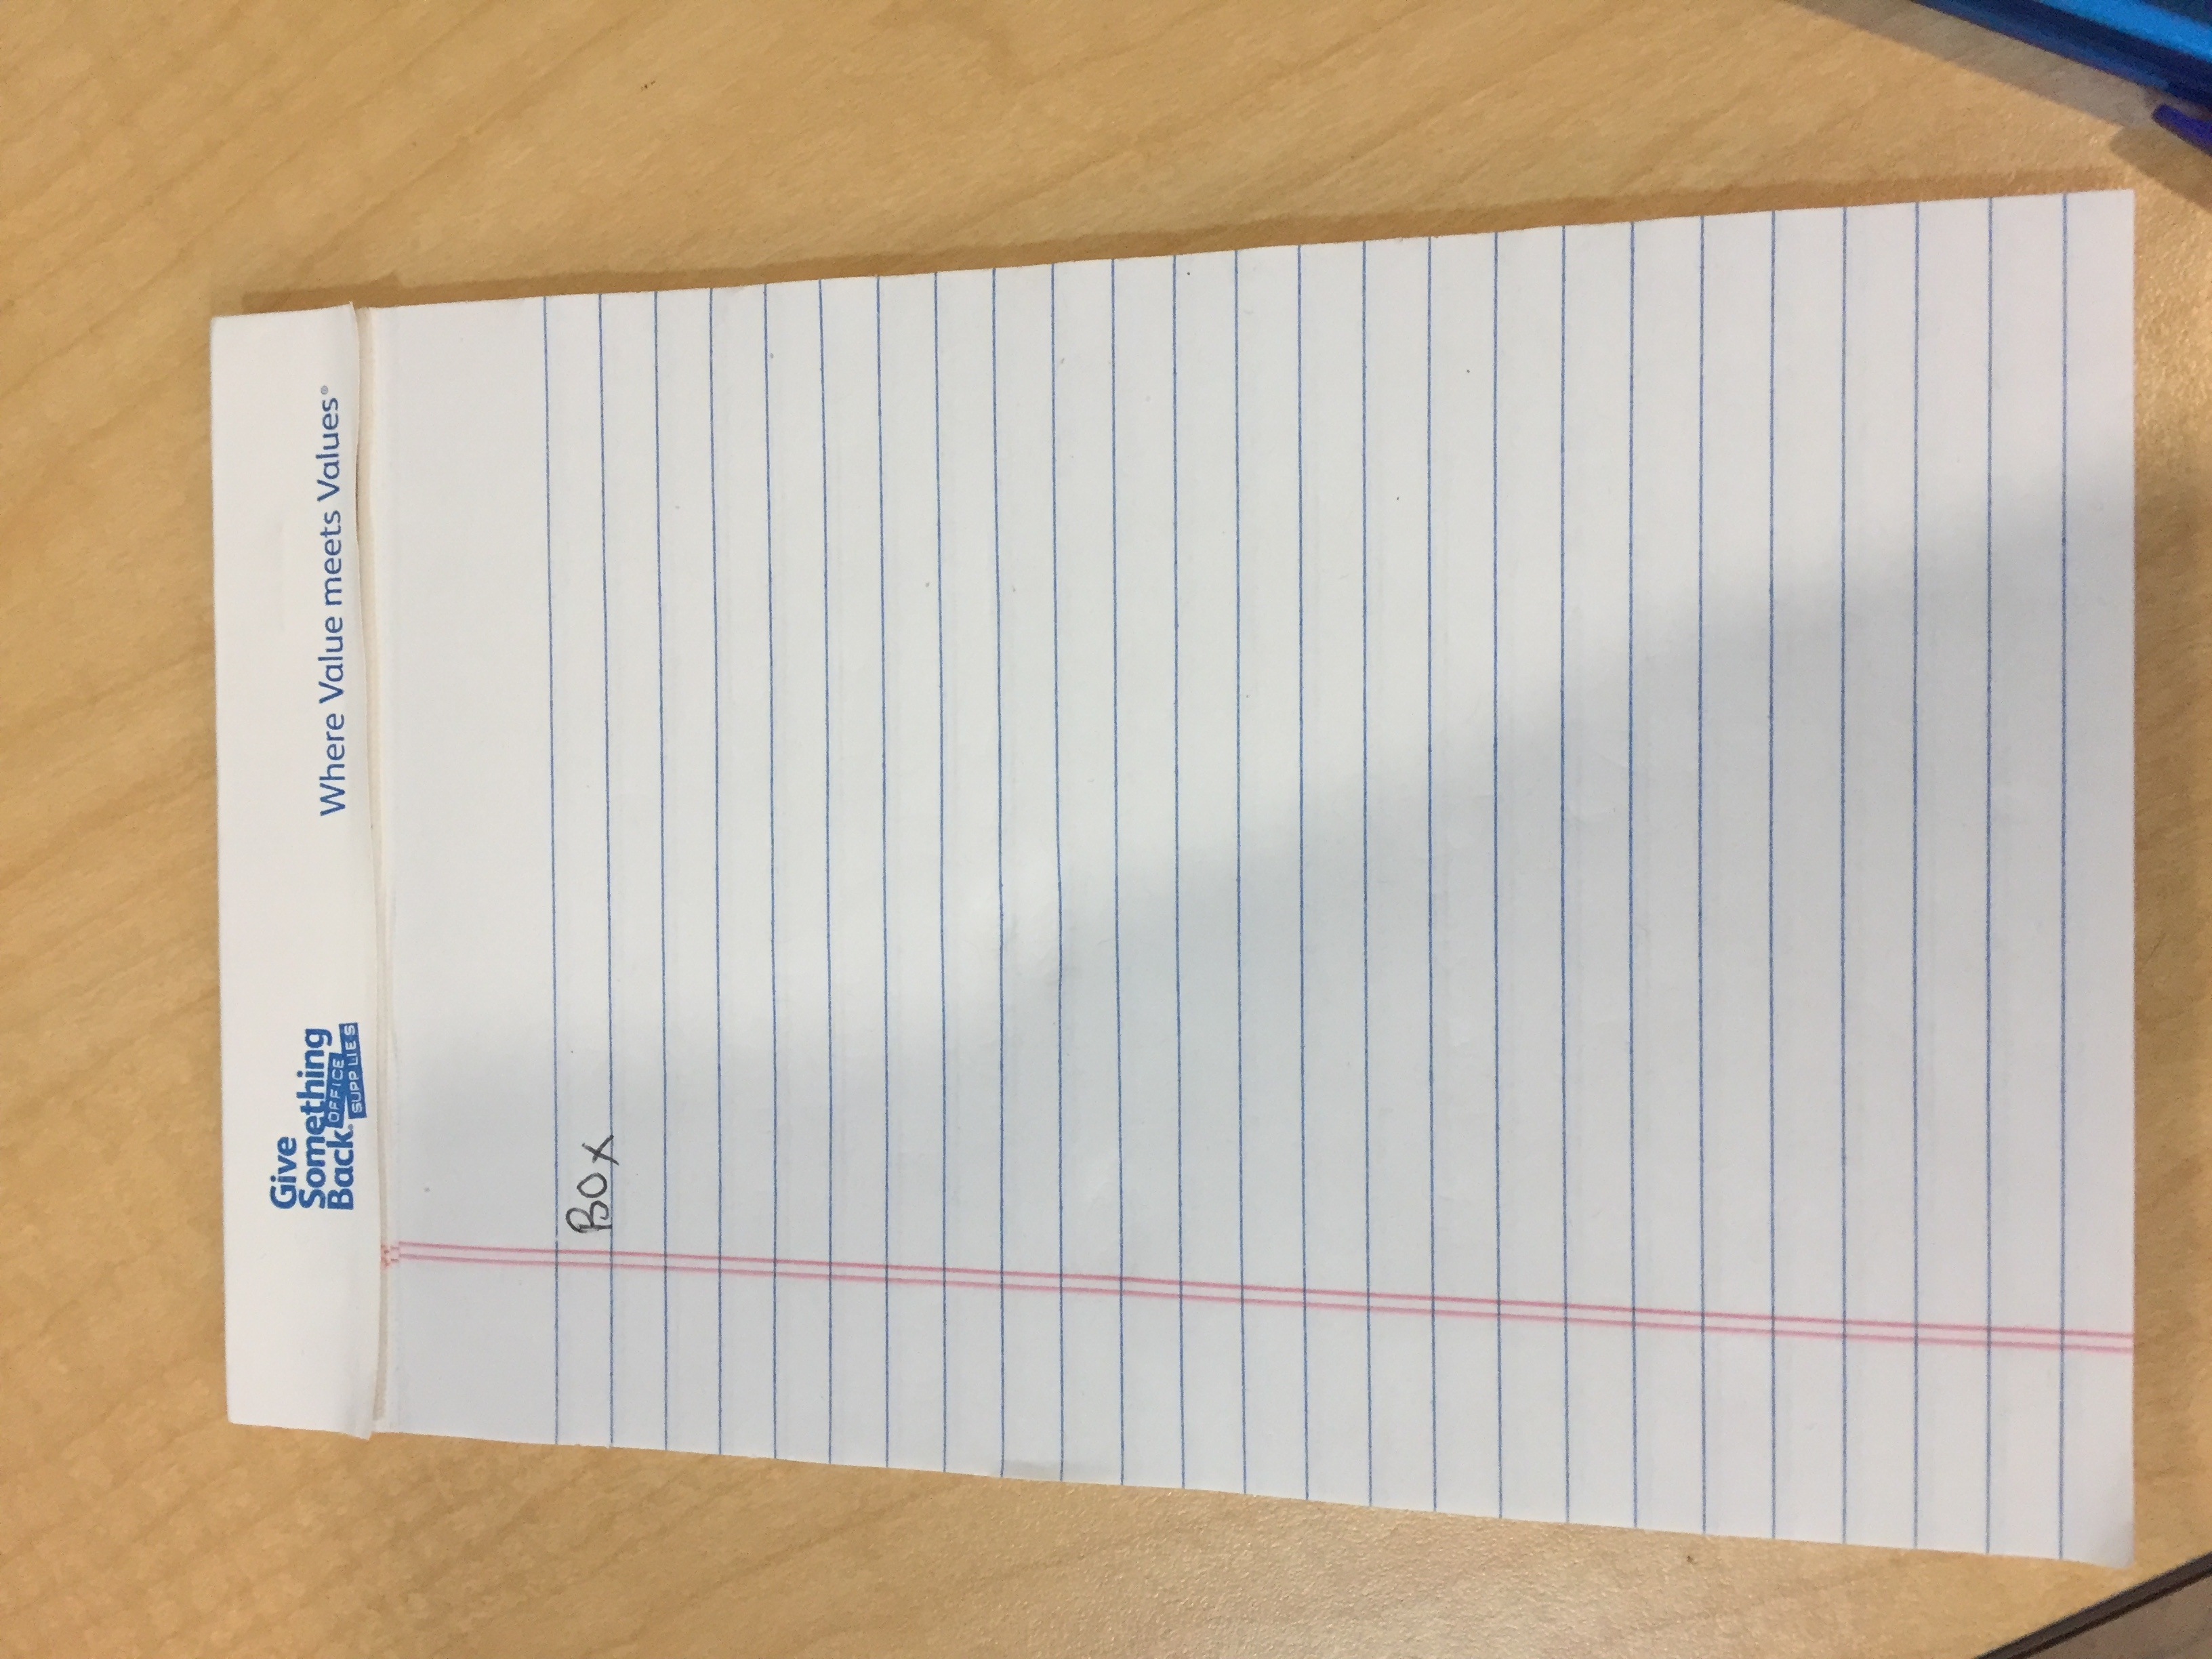
\includegraphics[scale=0.10]{img/perspective/input.JPG}
    \caption{Начальное изображение}
    \label{input}
\end{figure}

Для начала необходимо удалить текст с изображения. Для этого преобразуем изображение в серый цвет и применим к нему размытие Гаусса \cite{gauss_blur}. На выходе данного этапа имеем изображение, представленное на рисунке ~\ref{gauss_blur}

\begin{figure}
    
\includegraphics[scale=0.5]{img/perspective/blured.png}
    \caption{Изображение после размытия Гаусса}
    \label{gauss_blur}
\end{figure}

Для поиска контуров необходимо выделить ребра. Для этого используется алгоритм Канни \cite{canny}. На выходе имеем изображение, представленное на рисунке ~\ref{canny}
\begin{figure}
    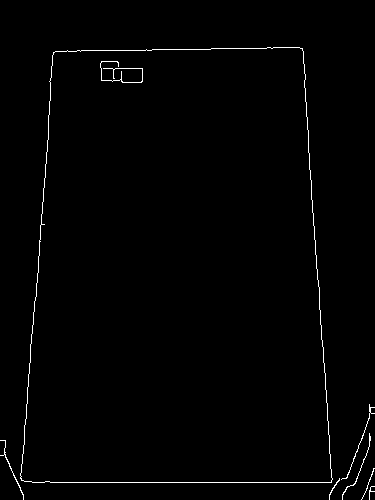
\includegraphics[scale=0.5]{img/perspective/canny.png}
    \caption{Ребра, найденные на изображении}
    \label{canny}
\end{figure}

После нахождения ребер поиск контуров осуществляется двумя способами:
\begin{enumerate}
    \item С помощью алгоритма $Line Segment Detector$ \cite{lsd}
    \item С помощью встроенного в $openCV$ алгоритма поиска контуров \cite{opencv_contours}
\end{enumerate}

Опишем подробнее поиск контуров на основе найденных линий: после прохода алгоритма имеем изображение, представленное на рисунке ~\ref{lsd_img}
\begin{figure}
    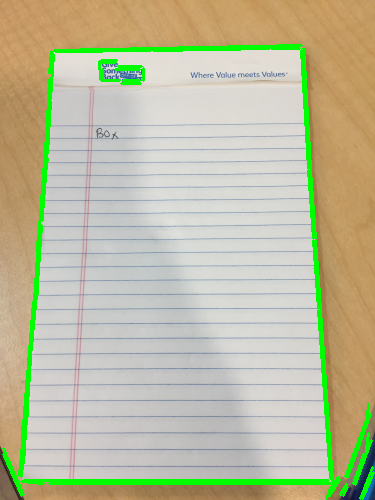
\includegraphics[scale=0.5]{img/perspective/lsd.png}
    \caption{Найденные на изображении линии с помощью алгоритма $LSD$}
    \label{lsd_img}
\end{figure}

Контур определяется как пересечение горизонтальных и вертикальных линий. На выходе имеем найденные углы контура, показанные на рисунке ~\ref{lsd_corners}
\begin{figure}
    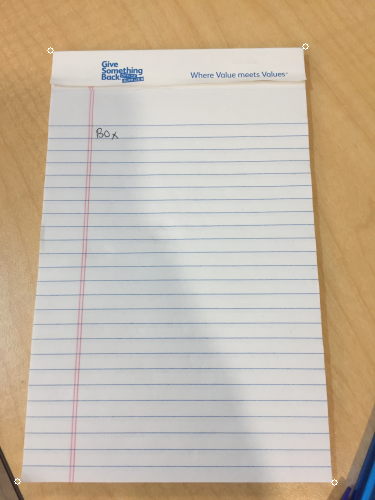
\includegraphics[scale=0.5]{img/perspective/corners.png}
    \caption{Найденные на изображении контуры на основе линий}
    \label{lsd_corners}
\end{figure}

С помощью библиотеки $openCV$ контуры находятся следующим образом:

\begin{enumerate}
    \item Находятся 5 наибольших по площади контуров
    \item Найденные контуры проверяются на количество углов, минимальную площадь контура
\end{enumerate}

Среди всех подходящих контуров выбирается наибольший по площади, как показано на рисунке ~\ref{contours}
\begin{figure}
    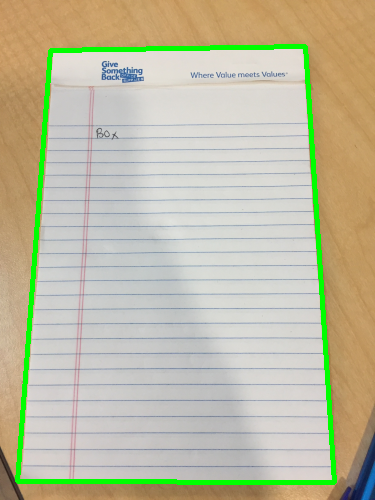
\includegraphics[scale=0.5]{img/perspective/contours.png}
    \caption{Найденные алгоритмом контуры}
    \label{contours}
\end{figure}


На основе найденного контура, представляющего лист бумаги, осуществляем коррекцию перспективы. Для этого находим матрицу коррекции \cite{opencv_perspective_transform} и примянем ее к изображению \cite{opencv_warp_perspective}.
Получаем результирующее изображение, показанное на рисунке ~\ref{perspective_correction}
\begin{figure}
    \includegraphics[scale=0.1]{img/perspective/perspective.png}
    \caption{Изображение с коррекцией перспективы}
    \label{perspective_correction}
\end{figure}

Далее необходимо добавить эффект сканирования. Эффект достигается путем применения к композиции небольшого размытия и серого изображения алгоритма сегментации $Adaptive Threshold$ \cite{opencv_threshold}. 
В конечном итоге имеем результирующее изображение показанное на рисунке ~\ref{preprocess_out}

\begin{figure}
    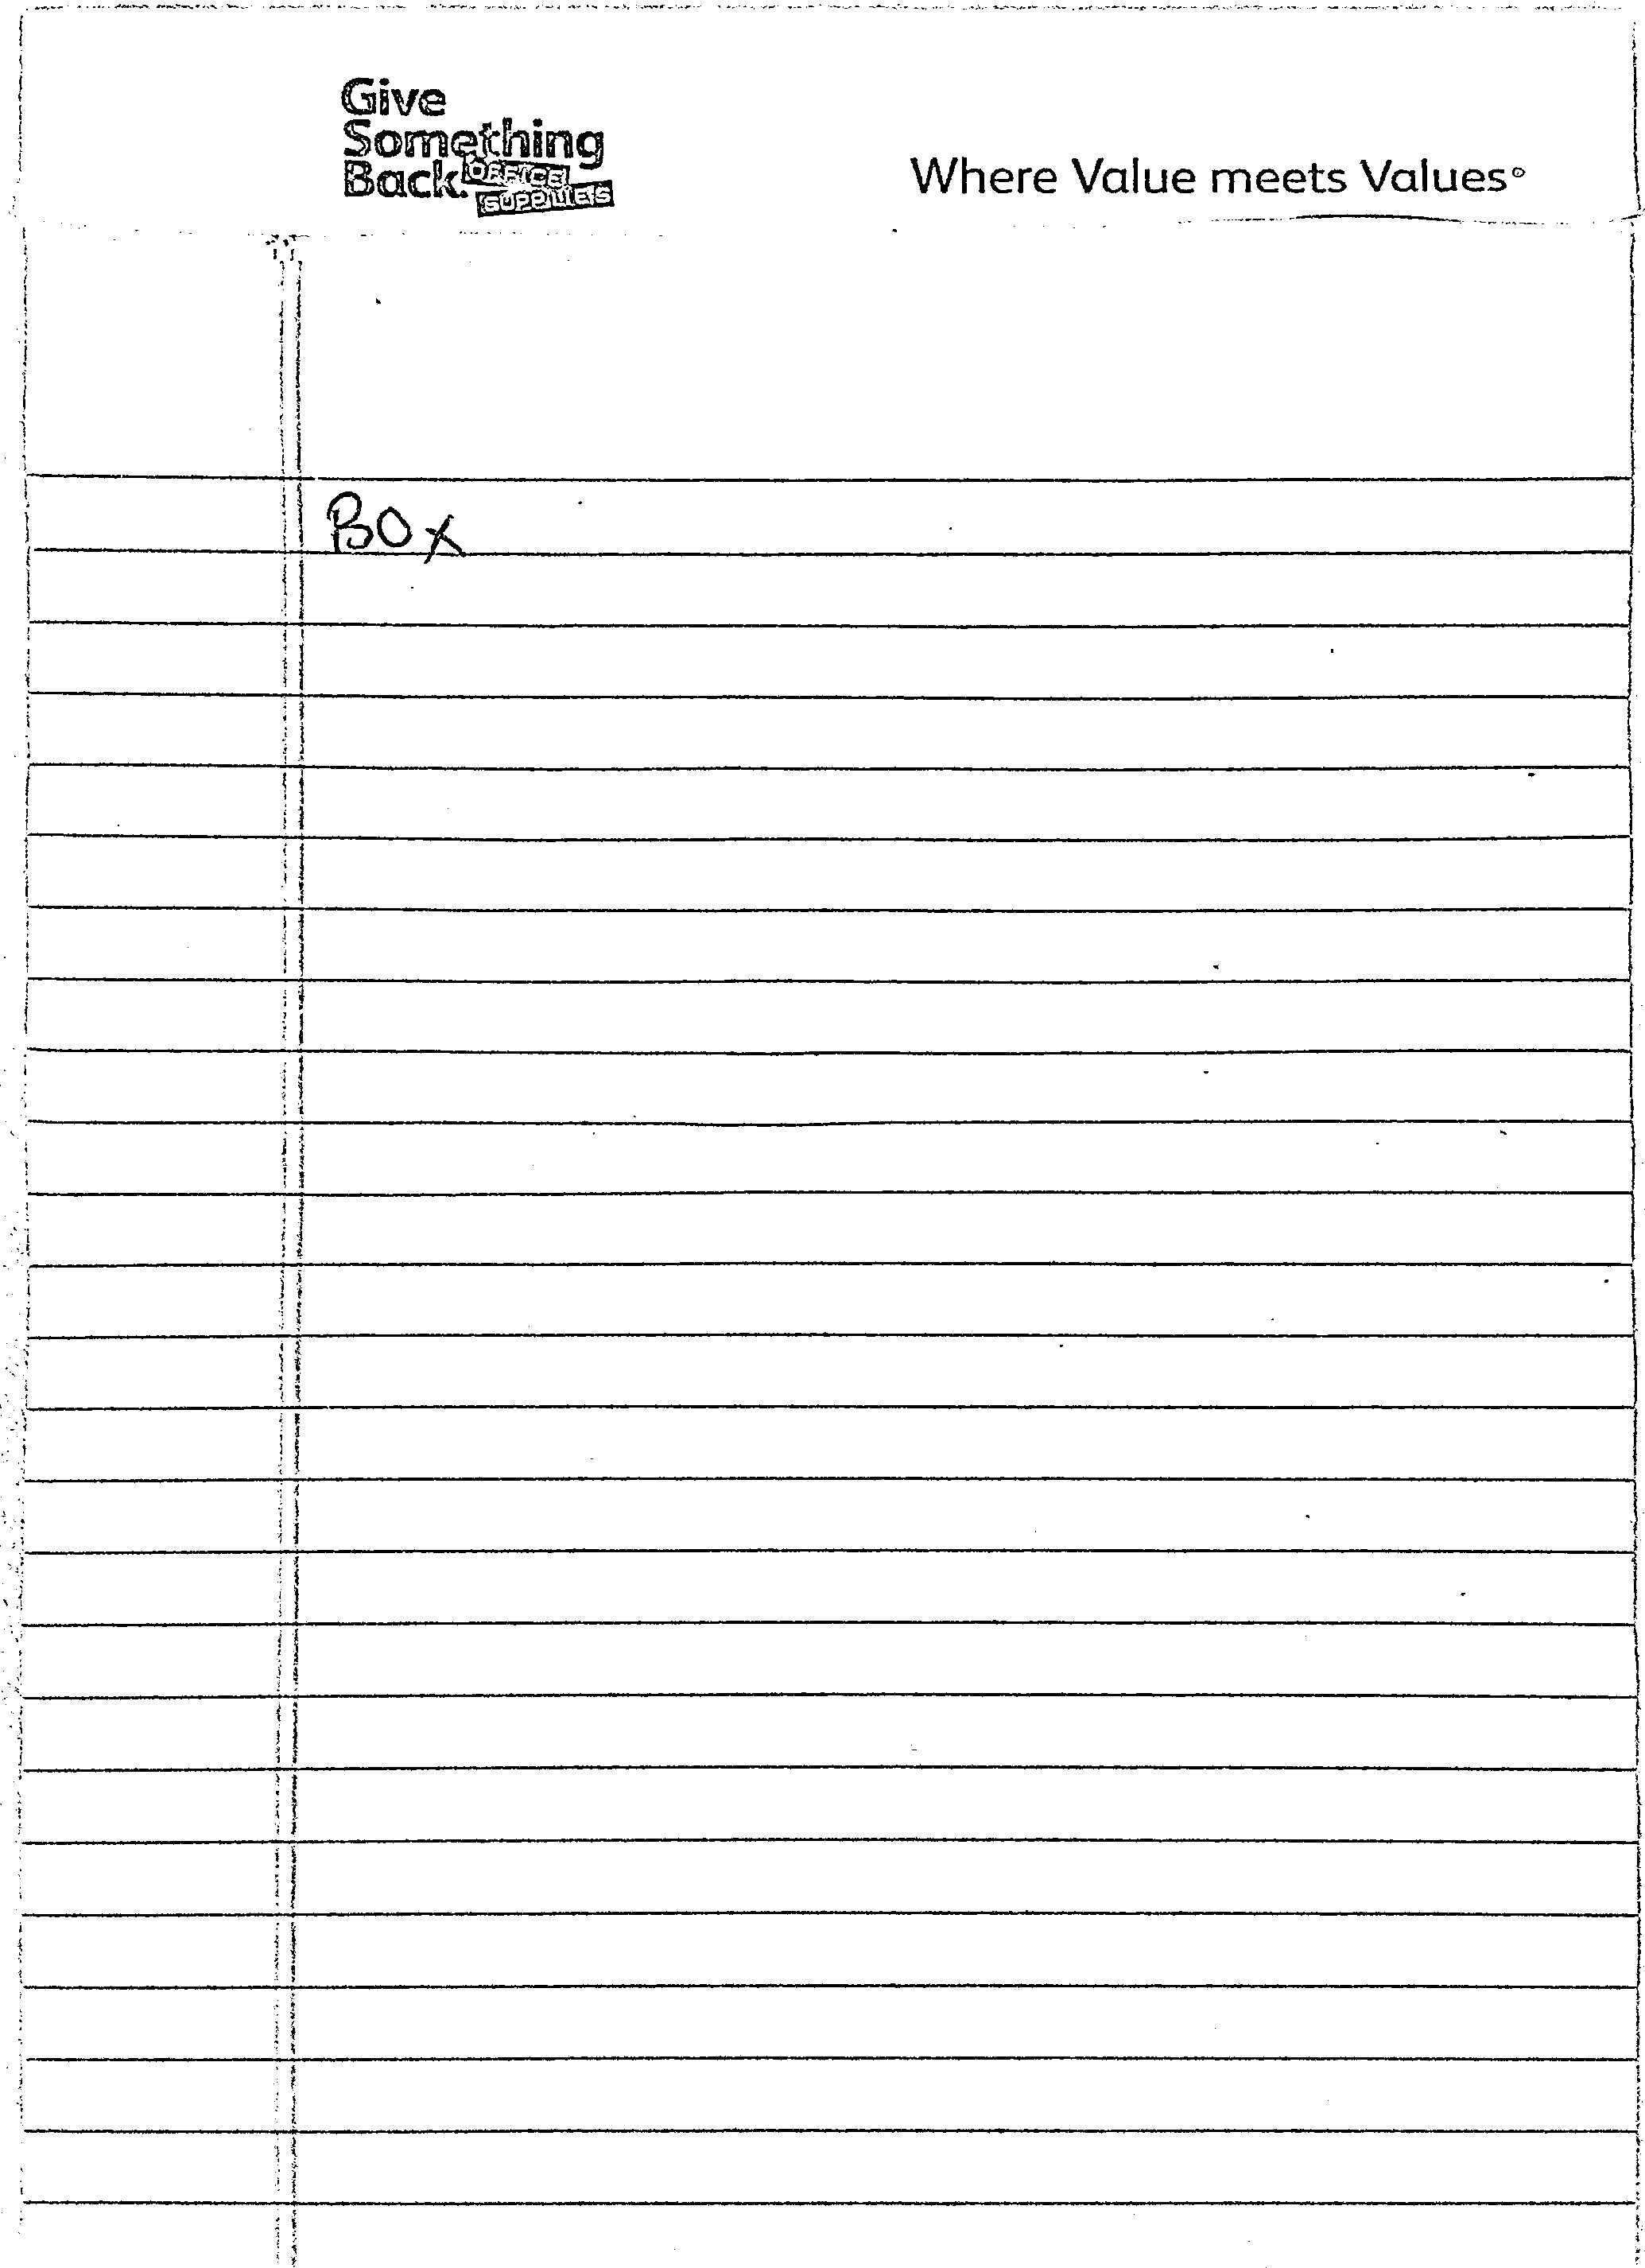
\includegraphics[scale=0.15]{img/perspective/output.JPG}
    \caption{Результирующее изображение}
    \label{preprocess_out}
\end{figure}

\subsubsection{Неправильное распознавание}
Стоит отметить, что данный алгоритм не является ультиимативным. Например, если на изображении находится посторонний шум (например, палец на бумаге, экран монитора, большое здание в виде прямоугольника), 
то алгоритм не сможет найти или найдет неверный контур. Именно с целью защиты от таких случаев в конечном продукте пользователь должен удостовериться в правильности найденного контура и отредактировать границы контура при необходимости.
Пример входного изображения, дающего неверный результат, и найденные на нем контуры приведены на рисунках ~\ref{perspective_wrong_input} и ~\ref{perspective_wrong_output} соответственно.

\begin{figure}
    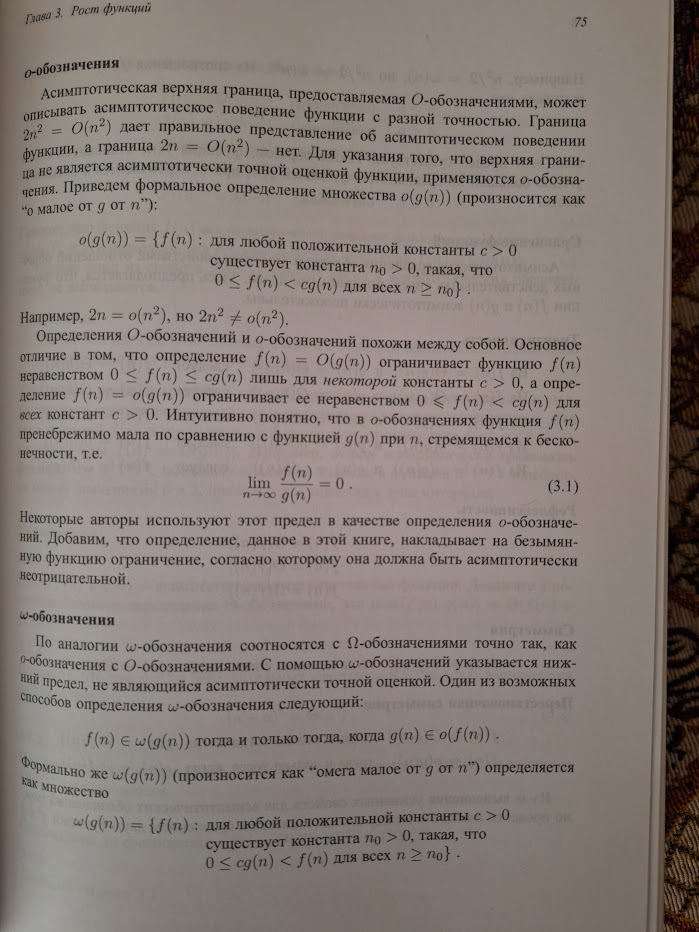
\includegraphics[scale=0.15]{img/perspective/wrong_input.JPG}
    \caption{Пример неправильно распозного изображения: входное изображение}
    \label{perspective_wrong_input}
\end{figure}

\begin{figure}
    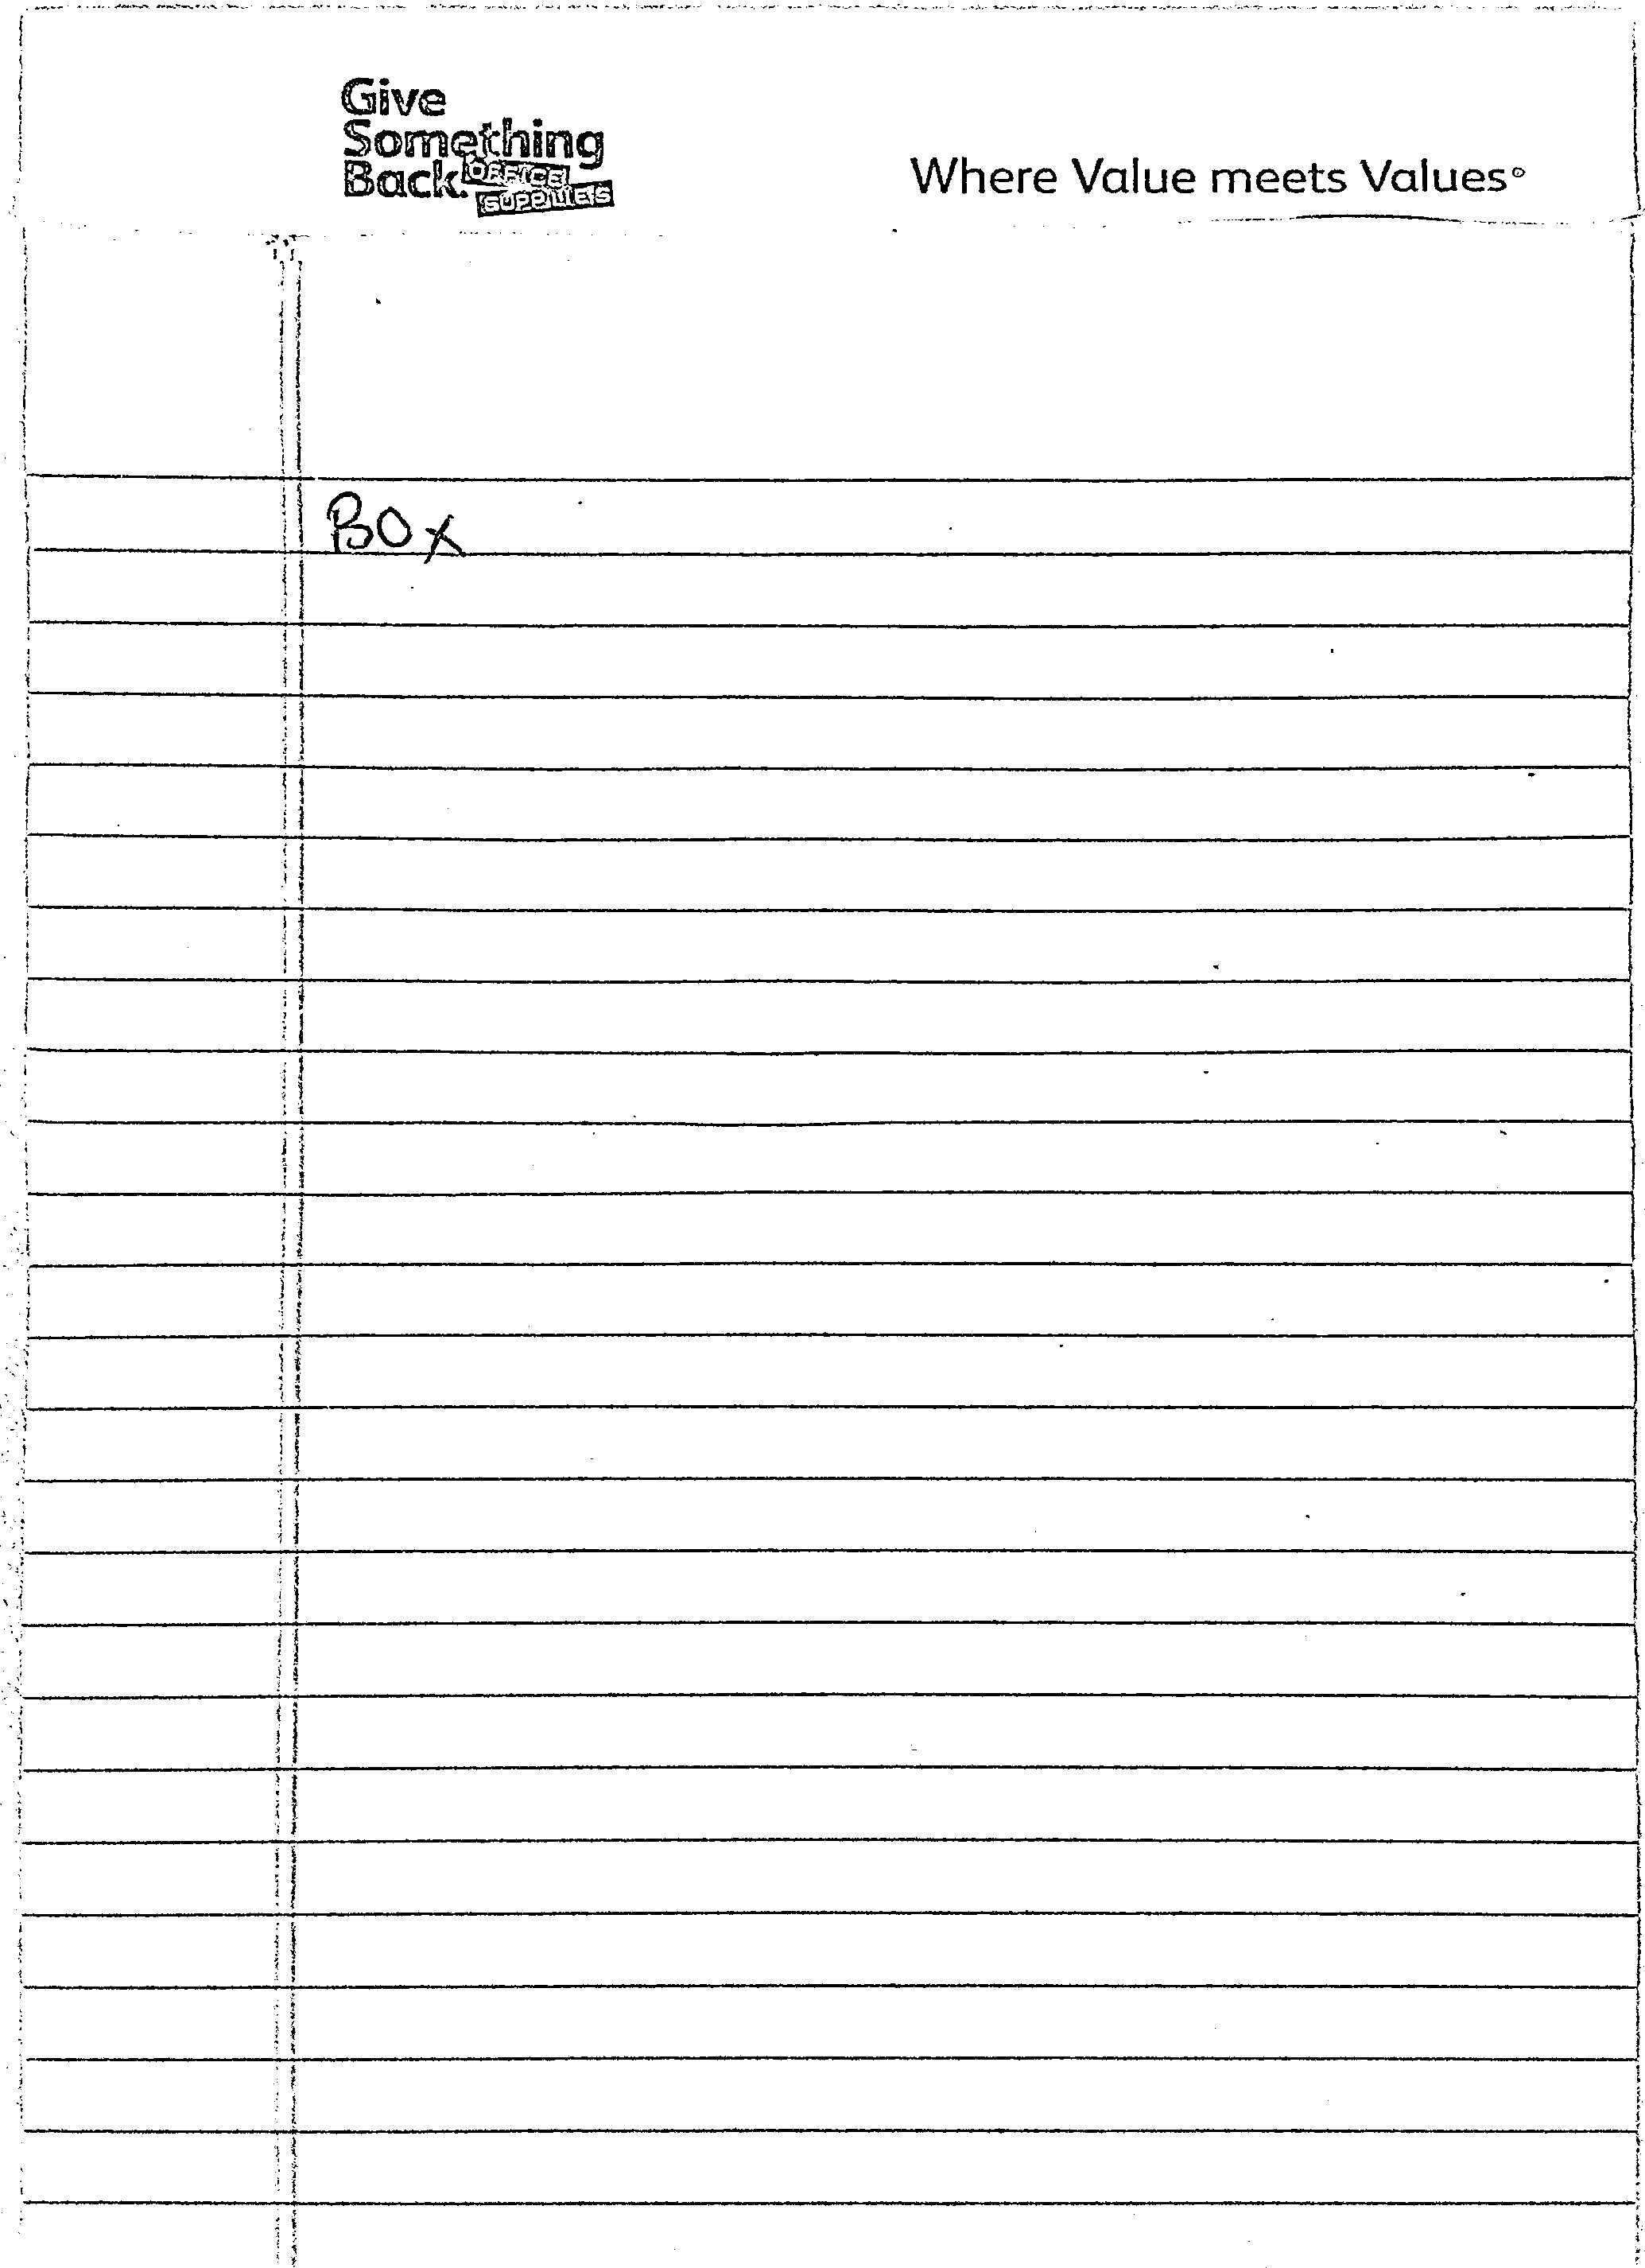
\includegraphics[scale=0.15]{img/perspective/wrong_output.JPG}
    \caption{Пример неправильно распозного изображения: найденные контуры}
    \label{perspective_wrong_output}
\end{figure}

\subsection{Сегментация}

Сегментация состоит из двух отдельных этапов:
\begin{itemize}
    \item Сегментация на абзацы
    \item Отделение текста от формул, рисунков и пр.
\end{itemize}

\subsubsection{Сегментация на абзацы}

Выделение абзацев требуется для их дальнейшего сохранения в \LaTeX\; коде. Данный вид сегментации, как и коррекция перспективы, осуществляется исключительно алгоритмически.
Поэтому данный этап можно также исполнять на машине пользователя.

%TODO: расписать сегментацию на абзацы
%TODO: Добавить пример неправильной сегментации

\subsubsection{Выделение формул}

Для выделения формул недостаточно одних алгоритмов обработки изображений. Существует множество моделей, выполняющих распознование объектов на изображении.
Одной из таких моделей является $YOLO$. Данная модель обладает следующими преимуществами:
\begin{itemize}
    \item Быстродействие. Нейросеть работает в реальном времени, поэтому её используют для распознавания объектов на фото и видео "здесь и сейчас".
    \item Точность. Нейросеть $YOLO$ умеет распознавать объекты разных размеров в пределах одного кадра.
    \item Универсальность. Нейросеть $YOLO$ способна определять как хорошо знакомые ей объекты, так и те, с которыми она ещё не сталкивалась.
    \item Простота. Модель $YOLO$ можно запросто запускать и дообучать с помощью $Tensorflow$.
\end{itemize}

Однако, данная модель не специализирована на какой-то одной задаче, поэтому будет проигрывать специализированным моделям.

На основании плюсов данной модели, а также на основании самой архитектуры системы, позволяющую при необходимости легко заменить выбранную модель на другую, было принято решение использовать для распознования формул модель $YOLO$ последней версии $v8$.

\subsubsection{Обучающие данные}
 % Глава 2
% \include{contents/chapter-3} % Глава 3

% \conclusion

В результате выполнения выпускной квалификационной работы бакалавра была разработана система, выполняющая распознование научного текста и генерацию его \LaTeX\; кода. Были решены следующие задачи:

\begin{itemize}
    \item опредены пользовательские сценарии;
    \item определены требования к платформе;
    \item спроектирована архитектура платформы;
    \item спроектирован и разработан рабочий прототип платформы;
    \item произведено тестирование прототипа на реальном изображении.
\end{itemize}

Развитие данной платформы, спроектированной и реализованной в данной работе, может позволить перевести существующие отсканированные документы в оцифрованный вид. На данном этапе платформа не способна конкурировать с аналогичными решениями, например, $Mathpix$ \cite{mathpix}.

Для успешного конкурирования необходимо улучшить качество распознования формул, поддержать распознование изображений в тексте, добавить распознование рукописного текста, научиться распозновать структуру текста (заголовки, списки, выделение курсивом, полужирным и пр.). % Заключение

\printbibliography % Список литературы

\appendix % Приложения
% \include{contents/appendix-qr}
\end{document}